\pagebreak
\subsubsection{Use Cases}

\begin{itemize}
	\item UC1: A user can view real time data gathered from a patient.

	\item UC2: A user can view historical data detailing a period of time.
	
	\item UC3: A user can view statistical data from over a period of time.

	
	\item UC4: A user can register to create an account and link to a particular patient.
	
	\item UC5: A user can log in to his or her account.
	
	\item UC6: A user can log out of his or her account.
	
	\item UC7: A user can manage his or her account information.		

	\item UC8: An admin user can manage other users' access rights.


	\item UC9: A user, caregiver, or doctor can get notifications if something is wrong according to the data.

	
	\item UC10: A user can see all previous notifications.

	\item UC11: A user can view general advice on the App.
	
	\item UC12: A user can add or remove medical persons' contact details to the app.

	\item UC13: A user can configure devices remotely.

		
	\item UC14: A researcher can view the data in the database anonymously.	
	

\end{itemize}
\pagebreak
\begin{figure}[!htb]
	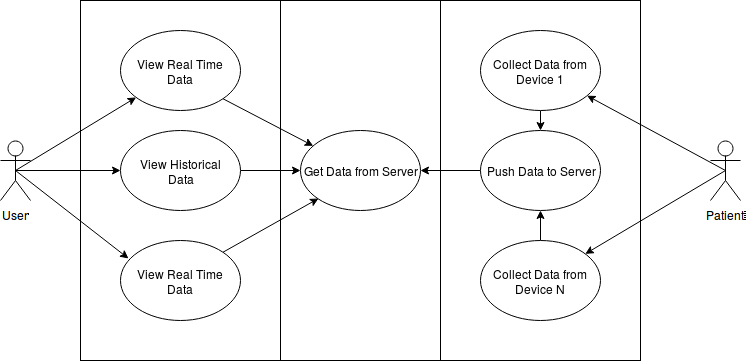
\includegraphics[width=15cm, height=7cm]{Diagrams/UseCase123.png}
	\caption{UC1, UC2, UC3}
\end{figure}

\pagebreak

\begin{figure}[!htb]
	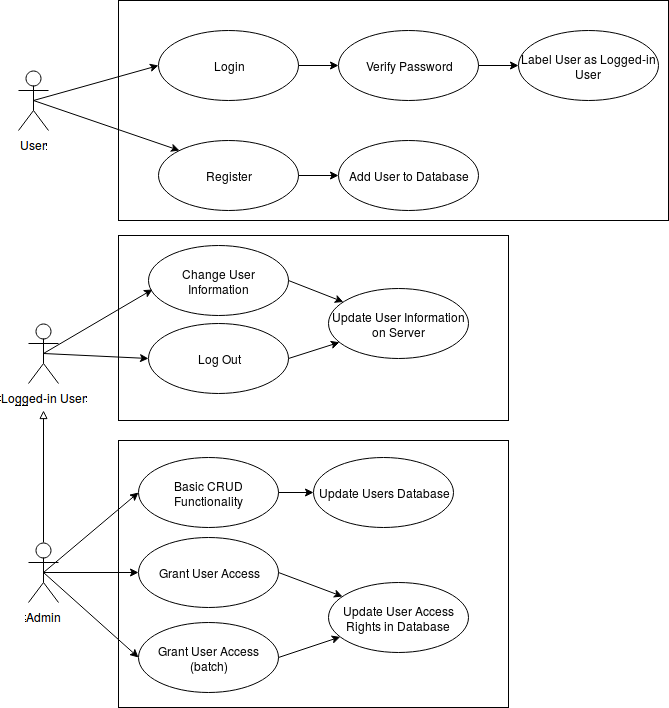
\includegraphics[width=15cm, height=15cm]{Diagrams/UseCase45678.png}
	\caption{UC4, UC5, UC6, UC7, UC8}
\end{figure}

\pagebreak

\begin{figure}[!htb]
	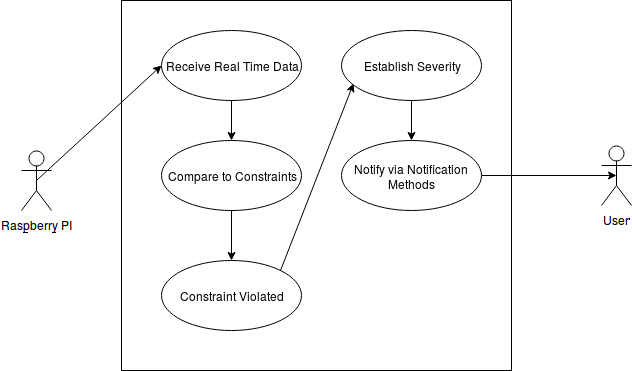
\includegraphics[width=15cm, height=7cm]{Diagrams/UseCase4.png}
	\caption{UC9}
\end{figure}

\begin{figure}[!htb]
	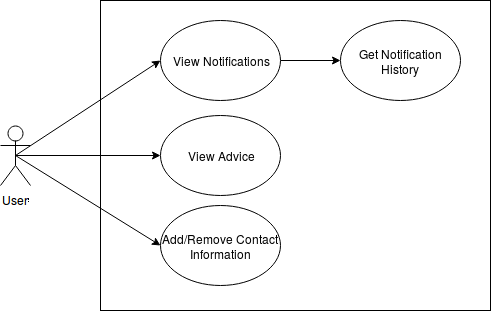
\includegraphics[width=15cm, height=7cm]{Diagrams/UseCase101112.png}
	\caption{UC10, UC11, UC12}
\end{figure}

\pagebreak

\begin{figure}[!htb]
	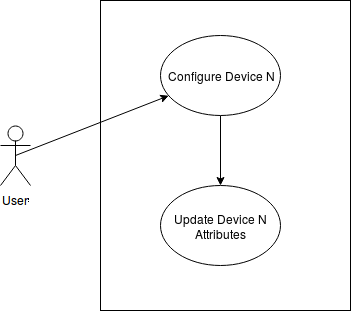
\includegraphics[width=10cm, height=7cm]{Diagrams/UseCase13.png}
	\caption{UC13}
\end{figure}

\pagebreak